%https://claude.ai/chat/9d70f2ed-b35f-476f-ae38-18ab56af1d1d


\documentclass[10pt]{article}

\title{On the viral proliferation of the black body process}
\author{S. Halayka\footnote{sjhalayka@gmail.com}}


\date{\today\;\currenttime}

\usepackage{datetime}
\usepackage{listings}
\usepackage{cite}
\usepackage{xcolor}
\usepackage{graphicx}
\usepackage{setspace}
\usepackage{amsmath}
\usepackage{amssymb}
\usepackage{amsthm}
\usepackage{url}
\usepackage[margin=0.8in]{geometry}
\usepackage{listings}
\usepackage{derivative}
\usepackage[]{lineno}

\usepackage{xcolor}
\usepackage{amsmath, amssymb}
\usepackage{bm}



\newtheorem{proposition}{Proposition}
\newtheorem{lemma}{Lemma}
\newtheorem{corollary}{Corollary}
\theoremstyle{definition}
\newtheorem{definition}{Definition}
\theoremstyle{remark}
\newtheorem{remark}{Remark}

%\doublespace




\begin{document}
\linenumbers


 
\maketitle

\begin{abstract}
This paper contains a self-contained and mathematically explicit introduction to gravitation and to the way that time dilation is currently understood. We derive Planck's law from the statistics of the radiation field, obtain Wien's displacement law and the Stefan--Boltzmann law as corollaries, and present the limiting (Rayleigh--Jeans and Wien) regimes. We then derive the general-relativistic deflection of starlight at the limb of the Sun directly from the Schwarzschild null geodesics, contrasting it with the Newtonian prediction. The thermodynamics and time dilation of the Kerr black hole are derived from the Kerr metric. Finally, these strands are unified through a precisely stated \emph{exogeneity--endogeneity} framework, and a unique perspective regarding the proliferation of the black body process is given: as kinematic and/or gravitational time dilation become extreme, the time rate of a body tends to zero, its internal (endogenous) process is interrupted, and the body asymptotes to a pure black body. We argue that this ``black body process'' is contagious in a sense that we make quantitative.
\end{abstract}

\section{Introduction}

\subsection{Conventions and units}

Throughout this paper we generally use \emph{Planck units}, in which the reduced Planck constant $\hbar$, the speed of light $c$, the gravitational constant $G$, and the Boltzmann constant $k_B$ are all set equal to unity:
\begin{equation}
\hbar = c = G = k_B = 1.
\end{equation}
In these units mass, length, time, and temperature are all measured in the same dimensionless system, and every physical quantity becomes a pure number expressed as a multiple of the corresponding Planck quantity. We note for later use that, because Planck's (non-reduced) constant is $h = 2\pi\hbar$, the choice $\hbar = 1$ implies
\begin{equation}
h = 2\pi .
\end{equation}
This single fact is responsible for the factors of $2\pi$ that appear in the black-body formulae below. The metric signature is taken to be $(-,+,+,+)$, and Greek indices run over the four spacetime coordinates. We restore SI factors only when reporting numbers that are to be compared with observation.

\subsection{Outline}

First we discuss Planck's law, the black body spectrum, and spectrography, deriving each of the standard results (Planck's law, the Rayleigh--Jeans and Wien limits, Wien's displacement law, and the Stefan--Boltzmann law) explicitly. Next we discuss the deflection of starlight by the Sun's gravitation, obtaining the famous factor of two over the Newtonian value from the Schwarzschild geodesic equation. We then derive the horizon structure, Hawking temperature, and time dilation of the Kerr black hole. Finally, we piece all of these concepts together when considering the proliferation of the black body process, which we phrase as a quantitative statement about the combined time rate $\eta$ and the exogeneity $e_x$ that we define below.




\section{Planck's law and spectrography}

A black body is an idealized physical object that absorbs all incident electromagnetic radiation, regardless of frequency or angle of incidence, and re-emits radiation in a characteristic spectrum that depends only on its temperature. Although no perfect black body exists in nature, many objects approximate this behavior closely enough that the model is extraordinarily useful: stars, heated cavities, and the cosmic microwave background are all well described, to a good approximation, as black body emitters \cite{rybicki}.

\subsection{Statement of Planck's law}

The spectral radiance of a black body at temperature $T$ is given by Planck's law \cite{planck}. Expressed as a function of wavelength $\lambda$, in the Planck units fixed above,
\begin{equation}\label{eq:planck-lambda}
B_\lambda(\lambda, T) = \frac{4 \pi}{\lambda^5} \cdot \frac{1}{\exp\!\left(\dfrac{2 \pi}{\lambda T}\right) - 1}.
\end{equation}
The quantity $B_\lambda$ is the power emitted per unit area of the emitting surface, per unit solid angle, per unit wavelength interval. See Fig.~\ref{fig1}, where the spectral radiance for several example temperatures is drawn. Planck's law was introduced by Max Planck in 1900 and is widely regarded as the historical origin of quantum theory, since its derivation required the (then-radical) assumption that electromagnetic energy is exchanged in discrete quanta rather than continuously. Planck was awarded the Nobel prize for this work.

\subsection{Derivation from the statistics of the radiation field}

Although Planck's law is quoted above as a definition, it is not an arbitrary fit; it follows from counting the electromagnetic modes of a cavity and assigning to each mode its mean thermal energy. We sketch the derivation in full because the mode-counting picture, in which the field is a collection of independent oscillators, is the cleanest way to see why a perfect black body spectrum is structureless.

Consider radiation in thermal equilibrium inside a cubical cavity of side $L$ and volume $V = L^3$ with perfectly conducting walls. The allowed standing-wave modes have wavevectors $\mathbf{k}$ whose Cartesian components are quantized as $k_i = \pi n_i / L$ with $n_i \in \{1,2,3,\dots\}$. The number of modes with wavenumber magnitude up to $k$ is the volume of the positive octant of a sphere of radius $kL/\pi$ in $\mathbf{n}$-space, multiplied by two to account for the two independent polarizations of light:
\begin{equation}
N(k) = 2 \cdot \frac{1}{8}\cdot\frac{4}{3}\pi\!\left(\frac{kL}{\pi}\right)^{\!3} = \frac{V k^3}{3\pi^2}.
\end{equation}
Differentiating, the number of modes per unit volume with wavenumber in $[k, k+dk]$ is
\begin{equation}
g(k)\,dk = \frac{1}{V}\frac{dN}{dk}\,dk = \frac{k^2}{\pi^2}\,dk.
\end{equation}
With $c = 1$ the dispersion relation is $\omega = k$, so the density of modes per unit volume per unit angular frequency is simply $g(\omega) = \omega^2/\pi^2$.

Each mode is a harmonic oscillator of angular frequency $\omega$. In thermal equilibrium at temperature $T$, the photon occupation of a mode is governed by Bose--Einstein statistics with vanishing chemical potential (photon number is not conserved) \cite{bose1924,einstein1917}. The mean energy of a mode of angular frequency $\omega$, discarding the zero-point contribution that does not radiate, is
\begin{equation}\label{eq:mean-energy}
\langle E(\omega)\rangle = \frac{\omega}{\exp(\omega/T)-1},
\end{equation}
where in Planck units the quantum of energy is $\hbar\omega = \omega$ and the thermal scale is $k_B T = T$. The spectral energy density (energy per unit volume per unit angular frequency) is the product of the density of modes and the mean energy per mode,
\begin{equation}
u_\omega(\omega,T) = g(\omega)\,\langle E(\omega)\rangle = \frac{\omega^2}{\pi^2}\cdot\frac{\omega}{\exp(\omega/T)-1} = \frac{\omega^3}{\pi^2\!\left[\exp(\omega/T)-1\right]}.
\end{equation}
For an isotropic radiation field, the spectral radiance emerging from a surface is related to the energy density by $B = u/(4\pi)$ per unit solid angle, with one factor of $c=1$ converting energy density to flux. Hence
\begin{equation}
B_\omega(\omega,T) = \frac{1}{4\pi}\,u_\omega = \frac{\omega^3}{4\pi^3\!\left[\exp(\omega/T)-1\right]}.
\end{equation}
To express this per unit wavelength we change variables. With $c=1$ the angular frequency and wavelength are related by $\omega = 2\pi/\lambda$, so $\left|d\omega/d\lambda\right| = 2\pi/\lambda^2$, and conservation of radiated power, $B_\lambda\,d\lambda = B_\omega\,\left|d\omega\right|$, gives
\begin{equation}
B_\lambda = B_\omega\,\frac{2\pi}{\lambda^2}
= \frac{1}{4\pi^3}\left(\frac{2\pi}{\lambda}\right)^{\!3}\frac{1}{\exp(2\pi/\lambda T)-1}\cdot\frac{2\pi}{\lambda^2}
= \frac{4\pi}{\lambda^5}\cdot\frac{1}{\exp(2\pi/\lambda T)-1},
\end{equation}
which is precisely Eq.~\eqref{eq:planck-lambda}. The same calculation carried out with the constants restored returns the familiar SI form $B_\lambda = (2hc^2/\lambda^5)\,[\exp(hc/\lambda k_B T)-1]^{-1}$, and one checks that substituting $h = 2\pi$, $c = 1$, $k_B = 1$ reproduces the prefactor $2hc^2 \to 4\pi$.

\begin{remark}
The crucial structural feature of Eq.~\eqref{eq:planck-lambda} is that it depends on $\lambda$ and $T$ only through the single dimensionless combination $\lambda T$, up to the overall $\lambda^{-5}$ scaling. This scaling self-similarity is what makes Wien's displacement law and the Stefan--Boltzmann law inevitable, as we now show.
\end{remark}

\subsection{Limiting regimes}

\paragraph{Rayleigh--Jeans (long-wavelength) limit.} When $2\pi/\lambda T \ll 1$, i.e. when the photon energy is small compared to the thermal energy, the exponential may be expanded as $\exp(2\pi/\lambda T) - 1 \approx 2\pi/\lambda T$, and Eq.~\eqref{eq:planck-lambda} reduces to the classical Rayleigh--Jeans form \cite{rayleigh1900,jeans1905}
\begin{equation}
B_\lambda \;\xrightarrow{\;\lambda T \to \infty\;}\; \frac{4\pi}{\lambda^5}\cdot\frac{\lambda T}{2\pi} = \frac{2T}{\lambda^4}.
\end{equation}
This contains no quantum of action and diverges as $\lambda \to 0$; the integral of $B_\lambda$ over all wavelengths would be infinite. This is the ultraviolet catastrophe, the classical pathology that Planck's quantization removes.

\paragraph{Wien (short-wavelength) limit.} When $2\pi/\lambda T \gg 1$, the $-1$ in the denominator is negligible and
\begin{equation}
B_\lambda \;\xrightarrow{\;\lambda T \to 0\;}\; \frac{4\pi}{\lambda^5}\,\exp\!\left(-\frac{2\pi}{\lambda T}\right),
\end{equation}
which is Wien's original empirical law \cite{wien1896}, exhibiting the exponential suppression of high-frequency emission that the classical theory failed to predict. Planck's law interpolates smoothly between these two regimes.

\subsection{Wien's displacement law}

The wavelength $\lambda_{\max}$ at which $B_\lambda$ is maximal is found by setting $\partial B_\lambda/\partial\lambda = 0$. Writing $a \equiv 2\pi/T$ and $x \equiv a/\lambda$, we have $B_\lambda \propto \lambda^{-5}(e^{a/\lambda}-1)^{-1}$, and
\begin{equation}
\frac{\partial B_\lambda}{\partial\lambda} \propto -5\lambda^{-6}\frac{1}{e^{a/\lambda}-1} + \lambda^{-5}\frac{(a/\lambda^2)\,e^{a/\lambda}}{(e^{a/\lambda}-1)^2} = 0.
\end{equation}
Multiplying through by $\lambda^6(e^{a/\lambda}-1)^2$ and simplifying yields the transcendental equation
\begin{equation}\label{eq:wien-transc}
x\,e^x = 5\!\left(e^x - 1\right), \qquad\text{equivalently}\qquad x = 5\!\left(1 - e^{-x}\right),
\end{equation}
whose unique positive root is $x_\star \approx 4.965114$. Therefore
\begin{equation}
\lambda_{\max}\,T = \frac{a}{x_\star}\,T = \frac{2\pi}{x_\star} \approx 1.2655 \quad\text{(Planck units)},
\end{equation}
which is the statement that the peak wavelength is inversely proportional to temperature, i.e.\ Wien's displacement law \cite{wien1893}. Restoring constants, $\lambda_{\max} T = hc/(x_\star k_B) \approx 2.898\times 10^{-3}\,\mathrm{m\,K}$, the measured Wien displacement constant. The downward and rightward march of the peak with decreasing temperature is exactly the behavior shown in Fig.~\ref{fig1}: the $6000\,\mathrm{K}$ curve peaks in the visible, whereas the $3000\,\mathrm{K}$ curve peaks in the near infrared.

\subsection{The Stefan--Boltzmann law}

Integrating the spectral radiance over all wavelengths gives the total radiance. With the substitution $x = 2\pi/\lambda T$, so that $\lambda = 2\pi/(xT)$ and $d\lambda = -2\pi/(x^2 T)\,dx$,
\begin{equation}
B(T) = \int_0^\infty B_\lambda\,d\lambda
= \int_0^\infty \frac{4\pi}{\lambda^5}\frac{d\lambda}{e^{2\pi/\lambda T}-1}
= \frac{T^4}{4\pi^3}\int_0^\infty \frac{x^3\,dx}{e^x-1}.
\end{equation}
The remaining integral is a standard one (see Appendix~\ref{app:zeta}),
\begin{equation}\label{eq:zeta-integral}
\int_0^\infty \frac{x^3}{e^x-1}\,dx = \Gamma(4)\,\zeta(4) = 6\cdot\frac{\pi^4}{90} = \frac{\pi^4}{15},
\end{equation}
so that the total radiance integrated over wavelength is $B(T) = (T^4/4\pi^3)(\pi^4/15) = \pi T^4/60$. The radiant flux emitted from a Lambertian surface into the outward hemisphere is $F = \pi B$, giving the Stefan--Boltzmann law \cite{stefan1879,boltzmann1884}
\begin{equation}
F(T) = \sigma_{\mathrm{SB}}\,T^4, \qquad \sigma_{\mathrm{SB}} = \frac{\pi^2}{60} \quad\text{(Planck units)}.
\end{equation}
Restoring the constants reproduces $\sigma_{\mathrm{SB}} = 2\pi^5 k_B^4/(15 h^3 c^2) \approx 5.67\times 10^{-8}\,\mathrm{W\,m^{-2}\,K^{-4}}$. The total emitted power therefore grows as the fourth power of temperature, which is why the area under the curves in Fig.~\ref{fig1} increases so steeply with $T$.

\begin{figure} 
\centering
  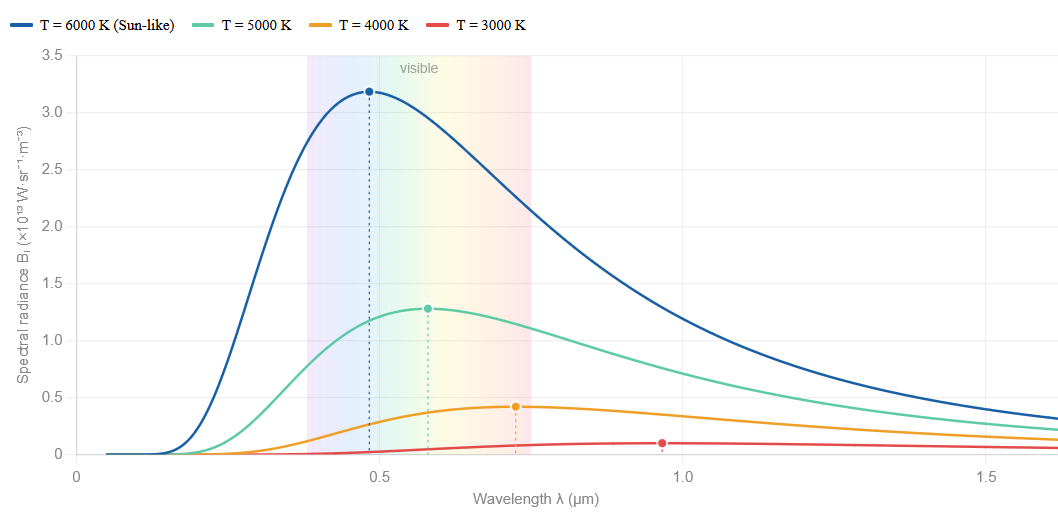
\includegraphics[width = 5 in]{wavelength.png}
  \caption{
A plot of spectral radiance (y axis) based on wavelength (x axis), for several example temperatures. The dotted markers indicate the peak wavelengths predicted by Wien's displacement law; the area under each curve scales as $T^4$ by the Stefan--Boltzmann law.
}
\label{fig1}
\end{figure}

\subsection{Gap-free spectra, and the spectrograph}

A perfect black body spectrum is gap-free: it represents pure thermal emission with no internal structure imprinted on the outgoing radiation. This is manifest in the derivation above: each cavity mode is statistically independent and carries the universal mean energy \eqref{eq:mean-energy}, so the emergent spectrum depends on nothing but $T$. Real bodies, by contrast, almost always show deviations from the ideal Planck curve, in the form of absorption or emission lines that reveal the internal composition and process(es) of the emitter. It is precisely this contrast --- between the perfect Planck spectrum and the line-rich spectra of real objects --- that motivates the discussion given in this paper.

A spectrograph shows which of the electromagnetic wavelengths are emitted (or not emitted) by a body for any given temperature. The gaps in the spectrum show that there are internal processes at those wavelengths --- like how the atmospheric content of the Sun blocks some light, resulting in the gaps (Fraunhofer lines) in the spectrum that we observe. We can make ``gap'' quantitative. If $I_0(\lambda)$ is the underlying continuum (the would-be black body intensity) and a cool intervening layer has optical depth $\tau(\lambda)$, then radiative transfer through the layer attenuates the continuum according to the Beer--Lambert law,
\begin{equation}
I(\lambda) = I_0(\lambda)\,e^{-\tau(\lambda)},
\end{equation}
and the depth and strength of an absorption line are summarized by its equivalent width
\begin{equation}\label{eq:equivalent-width}
W_\lambda = \int \left[1 - \frac{I(\lambda)}{I_0(\lambda)}\right] d\lambda = \int\left[1 - e^{-\tau(\lambda)}\right]d\lambda .
\end{equation}
A vanishing optical depth, $\tau \to 0$, returns the gap-free Planck spectrum $I = I_0$ and $W_\lambda = 0$; a large optical depth carves a saturated line into the continuum. The presence of structure in a real spectrum is therefore a direct measure of internal, endogenous process --- a notion we will sharpen in Section~\ref{sec:viral}. A sample spectrograph, with gaps, can be seen in Fig.~\ref{fig2}.

\begin{figure} 
\centering
  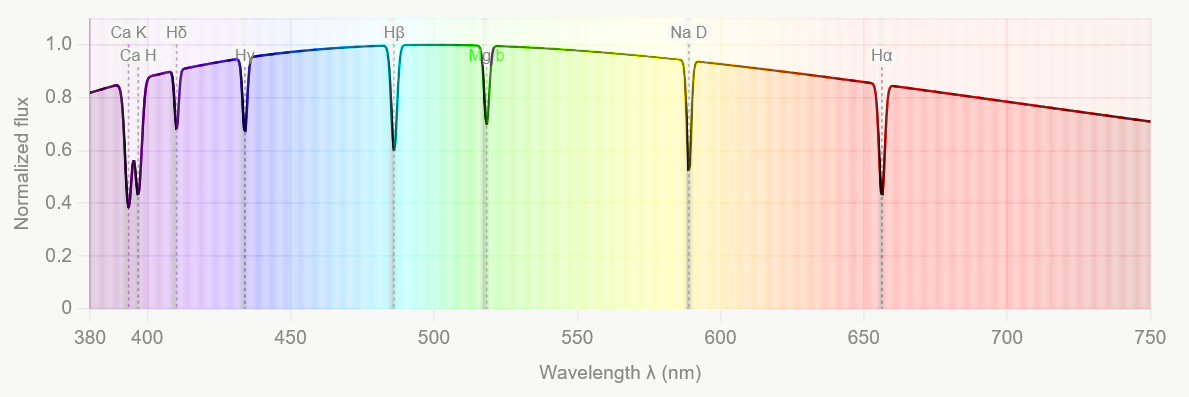
\includegraphics[width = 5 in]{gaps.png}
  \caption{
A sample spectrograph of the visible wavelengths, from the Sun, with Fraunhofer lines. Each labeled trough is an absorption line whose equivalent width \eqref{eq:equivalent-width} encodes the optical depth of the responsible species in the solar atmosphere.
}
\label{fig2}
\end{figure}






\section{Einstein's deflection of starlight at the limb of the Sun}

When light from a distant star passes close to the Sun on its way to Earth, the path of that light is bent by the Sun's gravitational field \cite{misner}. The angle of deflection $\alpha$, for a light ray that just grazes the limb of the Sun, is given by
\begin{equation}\label{eq:deflection}
\alpha = \frac{4 M_\odot}{R_\odot},
\end{equation}
where $M_\odot$ is the mass of the Sun, and $R_\odot$ is the radius of the Sun. We now derive this result, and the Newtonian result it doubles, from first principles.

\subsection{The Schwarzschild geometry and the orbit equation}

Outside a static, spherically symmetric mass $M$, spacetime is described by the Schwarzschild metric, which in the equatorial plane $\theta = \pi/2$ reads
\begin{equation}
ds^2 = -\left(1 - \frac{2M}{r}\right)dt^2 + \left(1 - \frac{2M}{r}\right)^{-1}dr^2 + r^2\,d\phi^2.
\end{equation}
The static and axial Killing vectors furnish two conserved quantities along a geodesic, the energy $E = (1-2M/r)\,\dot t$ and the angular momentum $L = r^2\dot\phi$, where the overdot denotes differentiation with respect to an affine parameter. For a light ray the geodesic is null, $ds^2 = 0$, which after dividing through and using the conserved quantities gives the radial equation
\begin{equation}
\left(\frac{dr}{d\phi}\right)^{\!2} = \frac{r^4}{b^2} - r^2\left(1 - \frac{2M}{r}\right), \qquad b \equiv \frac{L}{E},
\end{equation}
with $b$ the impact parameter. Substituting $u = 1/r$ and differentiating with respect to $\phi$ converts this into the compact orbit equation
\begin{equation}\label{eq:orbit}
\frac{d^2 u}{d\phi^2} + u = 3M u^2 .
\end{equation}
The term on the right, proportional to $M$, is the general-relativistic correction; setting it to zero gives the equation of a straight line, as it must in flat space.

\subsection{Perturbative solution and the bending angle}

We solve Eq.~\eqref{eq:orbit} perturbatively in the small quantity $M/b$. At zeroth order the solution is the straight line
\begin{equation}
u_0(\phi) = \frac{\sin\phi}{b},
\end{equation}
which describes a ray with closest approach $b$ at $\phi = \pi/2$ and reaching infinity ($u=0$) at $\phi = 0$ and $\phi = \pi$. Writing $u = u_0 + u_1$ and keeping terms of first order, the correction obeys
\begin{equation}
\frac{d^2 u_1}{d\phi^2} + u_1 = 3M u_0^2 = \frac{3M}{b^2}\sin^2\phi = \frac{3M}{2b^2}\left(1 - \cos 2\phi\right).
\end{equation}
A particular solution is $u_1 = \frac{3M}{2b^2} + \frac{M}{2b^2}\cos 2\phi$, so that
\begin{equation}
u(\phi) = \frac{\sin\phi}{b} + \frac{M}{2b^2}\left(3 + \cos 2\phi\right).
\end{equation}
The asymptotic directions of the ray are the angles at which $u = 0$. Near $\phi = 0$ we set $u = 0$, approximate $\sin\phi \approx \phi$ and $\cos 2\phi \approx 1$, and solve
\begin{equation}
0 = \frac{\phi}{b} + \frac{M}{2b^2}(3+1) = \frac{\phi}{b} + \frac{2M}{b^2} \quad\Longrightarrow\quad \phi \approx -\frac{2M}{b}.
\end{equation}
By the symmetry of the orbit the outgoing asymptote is displaced by the same amount past $\phi = \pi$. The total deflection is the sum of the two displacements,
\begin{equation}
\alpha = \frac{2M}{b} + \frac{2M}{b} = \frac{4M}{b},
\end{equation}
and for a ray grazing the limb, $b \to R_\odot$, this is exactly Eq.~\eqref{eq:deflection}.




\subsection{The Newtonian value and the factor of two}

It is instructive to compare with the prediction of Newtonian gravity applied to a corpuscle moving at the speed of light. Treating the photon as a fast test particle on a hyperbolic orbit and computing the transverse impulse, one finds the Newtonian deflection
\begin{equation}
\alpha_{\mathrm{N}} = \frac{2M}{b},
\end{equation}
exactly half of the relativistic result. The missing factor of two is supplied entirely by the curvature of \emph{space} --- the spatial part of the Schwarzschild metric, encoded in the $(1-2M/r)^{-1}$ in $g_{rr}$ --- which Newtonian gravity, having a flat spatial geometry, cannot account for. Inserting the standard values into Eq.~\eqref{eq:deflection} yields
\begin{equation}
\alpha = \frac{4 G M_\odot}{c^2 R_\odot} \approx 8.49\times 10^{-6}\ \mathrm{rad} \approx 1.75\ \text{arcseconds},
\end{equation}
twice the Newtonian amount. In the interpretation developed in this paper, the doubling is read as the signature of a receiver --- the photon --- whose internal process is practically none: neutrinos and photons, having little to no internal process at all (respectively), have their paths bent twice (or almost as twice) as much as Newton's gravity predicts. In this reading, internal process forms a resistance to gravitation. See Fig.~\ref{fig3} for the depiction of the deflection of starlight by the Sun's gravitation.

Einstein was given the Nobel prize for his discovery of the relationship between photon energy and Planck's constant, and how it goes to explain the photoelectric effect. However, his launch to superstardom truly occurred when Eddington measured $\alpha$ during an eclipse, validating the framework of general relativity, and dethroning Newtonian gravity as king of the cosmos.

\begin{figure} 
\centering
  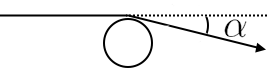
\includegraphics[width = 3 in]{deflection.png}
  \caption{
The Sun's gravitation bending the path of starlight. The grazing ray (impact parameter $b \approx R_\odot$) is deflected by $\alpha = 4M_\odot/R_\odot \approx 1.75''$, twice the Newtonian value.
}
\label{fig3}
\end{figure}








\section{The fundamental viral process}\label{sec:viral}

What we observe (or at least what we calculate out on paper) at levels of extreme time dilation is that a body becomes extremely external (exogenous, global), without internal (endogenous, local) process. The body becomes more and more like a black body as kinematic and/or gravitational time dilation kicks in. The purpose of this section is to make that statement precise. We first assemble the relevant time dilation factor --- and then define an exogeneity functional.

\subsection{The Kerr black hole}


For example, at extreme gravitational time dilation, you have a black hole, which is a black body emitting Hawking radiation \cite{schutz, hooft, jacobson, verlinde}. The rotating (Kerr) black hole is described, in Boyer--Lindquist coordinates, by the metric
\begin{equation}
ds^2 = -\left(1 - \frac{2Mr}{\Sigma}\right)dt^2 - \frac{4 M a r \sin^2\theta}{\Sigma}\,dt\,d\phi + \frac{\Sigma}{\Delta}\,dr^2 + \Sigma\,d\theta^2 + \left(r^2 + a^2 + \frac{2Ma^2 r\sin^2\theta}{\Sigma}\right)\sin^2\theta\,d\phi^2,
\end{equation}
where
\begin{equation}
\Sigma \equiv r^2 + a^2\cos^2\theta, \qquad \Delta \equiv r^2 - 2Mr + a^2, \qquad A \equiv (r^2 + a^2)^2 - a^2 \Delta \sin^2 \theta,
\end{equation}
and the rotation parameter (the angular momentum per unit mass) is
\begin{equation}
a = \frac{J}{M},
\end{equation}
with $J$ the black hole angular momentum and $M$ the black hole mass.

\paragraph{Horizons.} The event horizons are the surfaces of infinite redshift in the radial direction, where $g_{rr}\to\infty$, i.e. where $\Delta = 0$. Solving the quadratic $r^2 - 2Mr + a^2 = 0$ gives the inner and outer Kerr horizons
\begin{equation}\label{eq:horizons}
r_{\pm} = M \pm \sqrt{M^2 - a^2}.
\end{equation}
A horizon exists only for $a \le M$; the case $a = M$ is the extremal black hole, and $a > M$ would describe a naked singularity. The roots satisfy the useful relations $r_+ + r_- = 2M$ and $r_+ r_- = a^2$, from which
\begin{equation}\label{eq:identity}
r_+^2 + a^2 = r_+^2 + r_+ r_- = r_+(r_+ + r_-) = 2Mr_+ .
\end{equation}

\paragraph{Temperature.} The Hawking temperature is $T_\infty = \kappa/2\pi$, where $\kappa$ is the surface gravity of the outer horizon. For the Kerr solution the surface gravity is $\kappa = (r_+ - r_-)/[2(r_+^2 + a^2)]$, so the black hole temperature measured at infinity is
\begin{equation}\label{eq:kerr-temp}
T_\infty = \frac{1}{4\pi}\cdot\frac{r_+ - r_-}{r_+^2 + a^2} = \frac{1}{4\pi}\cdot\frac{\sqrt{M^2 - a^2}}{M r_+},
\end{equation}
where the second equality uses $r_+ - r_- = 2\sqrt{M^2-a^2}$ together with the identity \eqref{eq:identity}. Two limits are worth noting. For a non-rotating (Schwarzschild) hole, $a = 0$ gives $r_+ = 2M$ and the familiar $T_\infty = 1/(8\pi M)$, so that temperature falls as mass rises. For the extremal hole, $a \to M$ gives $T_\infty \to 0$: the maximally rotating black hole is cold, its emission shut off even as its horizon persists. The black hole is thus literally a black body, with a temperature fixed entirely by the external (exogenous) parameters $M$ and $a$ and no internal structure whatsoever --- the cleanest possible illustration of the theme of this paper.






\paragraph{Combined time dilation.} 

A moving observer measures a combined (kinematic and/or gravitational) time rate of
\begin{equation}\label{eq:sigma}
\eta = \frac{d\tau}{dt} = \sqrt{\frac{\Sigma\Delta}{A}
- \frac{\Sigma}{\Delta}\left(v^r\right)^2
- \Sigma\left(v^\theta\right)^2
- \frac{A\sin^2\theta}{\Sigma}\left(v^\phi - \frac{2Mar}{A} \right)^2},
\end{equation}
where the velocity components are given in spherical coordinates (e.g. $v^r = dr/dt$, $v^\theta = d\theta/dt$, $v^\phi = d\phi/dt$).
This factor lies in $[0,1]$ outside the ergosphere and vanishes on the static limit surface $r^2 - 2Mr + a^2\cos^2\theta = 0$, where the clock of the static observer freezes relative to infinity --- the endpoint of gravitational time dilation.





%\subsection{Kinematic time dilation}

%At (almost) extreme kinematic time dilation, there is no internal process, such as in the case of a light clock whose bouncing photon is swept almost entirely into translational motion. For an object moving with speed $v$ (with $c = 1$), the special-relativistic time rate is the reciprocal of the Lorentz factor,
%\begin{equation}\label{eq:kin-dilation}
%\frac{d\tau_k}{dt} = \sqrt{1 - v^2} = \frac{1}{\gamma},
%\end{equation}
%which again lies in $[0,1]$ and tends to $0$ as $v \to 1$.

%\subsection{The combined dilation}

%The two effects compose multiplicatively, since they act on independent factors of the metric and the boost. The combined proper-time rate is
%\begin{equation}\label{eq:sigma}
%\eta \equiv \frac{d\tau_g}{dt}\cdot\frac{d\tau_k}{dt} \in [0,1].
%\end{equation}
%Because each factor is bounded in $[0,1]$, so is their product; $\eta = 1$ corresponds to a static clock far from any mass, and $\eta = 0$ corresponds to extreme dilation of either kind --- at a horizon, on the static limit, or at the speed of light.




\subsection{The exogeneity--endogeneity functional}

We now formalize the central construction. The combined time rate $\eta$ measures how much of a body's coordinate-time evolution survives as proper time; its complement measures how much has been arrested by time dilation. We define the exogeneity and endogeneity accordingly.

\begin{definition}[Exogeneity and endogeneity]
For a body with the time rate $\eta \in [0,1]$, the \emph{exogeneity} $e_x$ is any quantity satisfying
\begin{equation}\label{eq:exogeneity}
e_x \geq 1 - \eta,
\end{equation}
and the \emph{endogeneity} is its complement
\begin{equation}\label{eq:endogeneity}
e_n = 1 - e_x.
\end{equation}
\end{definition}

The inequality \eqref{eq:exogeneity} expresses that the externally driven (exogenous) share of a body's behavior is at least the share of its time evolution that dilation has removed. The remainder $e_n$ is the internally driven (endogenous) share --- the internal process. We record the elementary but important consequences.

\begin{proposition}[Bounds]\label{prop:bounds}
For any $\eta \in [0,1]$ the exogeneity obeys $1 - \eta \le e_x \le 1$, and correspondingly $0 \le e_n \le \eta$.
\end{proposition}
\begin{proof}
The lower bound on $e_x$ is the definition \eqref{eq:exogeneity}. The upper bound follows from interpreting $e_x$ as a share, $e_x \le 1$, equivalently $e_n = 1 - e_x \ge 0$. Combining $e_n = 1 - e_x \le 1 - (1 - \eta) = \eta$ gives the stated bound on the endogeneity.
\end{proof}

\begin{proposition}[Black-body limit]\label{prop:bb-limit}
As the time dilation becomes extreme, $\eta \to 0$, the body becomes purely exogenous: $e_x \to 1$ and $e_n \to 0$.
\end{proposition}
\begin{proof}
By Proposition~\ref{prop:bounds}, $1 - \eta \le e_x \le 1$. Letting $\eta \to 0$ squeezes $e_x \to 1$, whence $e_n = 1 - e_x \to 0$.
\end{proof}

\begin{corollary}
At a black hole horizon or at the speed of light, the endogeneity vanishes: the body has no internal process and is, in this precise sense, a perfect black body.
\end{corollary}

\begin{remark}
The opposite regime, $\eta \to 1$, leaves $e_x$ only loosely constrained: the bound \eqref{eq:exogeneity} becomes $e_x \ge 0$, permitting a fully endogenous body ($e_n \to 1$). The framework is therefore asymmetric by design --- extreme dilation forces exogeneity, while its absence merely permits endogeneity. This asymmetry is the mathematical content of the claim that the black body process is something a body is driven \emph{toward}.
\end{remark}

\subsection{Process interruption and viral proliferation}

What good is this knowledge? It serves to show that time dilation is about internal process interruption. As $\eta$ decreases --- as a process goes faster, or sinks deeper into a gravitational well --- Proposition~\ref{prop:bb-limit} guarantees that the endogenous share $e_n \le \eta$ is squeezed toward zero, and whatever internal structure the body possessed (its absorption lines, its $\tau > 0$ in Eq.~\eqref{eq:equivalent-width}) is erased in favor of structureless, exogenously determined thermal emission. What kind of hijacking process is responsible for this? The black body process. The black body process is contagious; viral, in the sense that any body brought into a regime of extreme dilation --- by acceleration, by infall, or by proximity to a horizon --- is converted into a black body, and a black hole grown by accretion converts each infalling body in turn.

Process interruption is a concept taken from computer science \cite{intel}, where an external signal suspends the locally running computation and transfers control to a global handler. It seems to be not just an analogy, but rather the reality: the dilation factor $\eta$ plays the role of the fraction of local instructions that complete before the interrupt, and $e_x = 1 - e_n \ge 1 - \eta$ the fraction of control surrendered to the global, exogenous process.

It is this unification of the kinematic and gravitational time dilation --- both entering through the single bounded quantity $\eta$ of Eq.~\eqref{eq:sigma} --- which leads to the beginnings of a theory of quantum gravity that is based on the concept of the black body process. The faster a process goes, and/or the deeper into a gravitational field a process goes, the more the process becomes like the black body process.

\section{Conclusion}

We have given an explicit, self-contained derivation of the physics underlying a single conceptual claim. Planck's law was obtained from mode counting and Bose--Einstein statistics, and its corollaries --- the Rayleigh--Jeans and Wien limits, Wien's displacement law, and the Stefan--Boltzmann law --- were derived in the Planck-unit conventions used throughout. The deflection of starlight was computed from the Schwarzschild null geodesics, reproducing the observed $1.75''$ and exhibiting the factor of two over the Newtonian value as a consequence of spatial curvature. The Kerr horizons, Hawking temperature, and time dilation were read off the Kerr metric. Finally, the exogeneity--endogeneity framework was stated as precise definitions with proved bounds, and the central claim --- that extreme time dilation drives a body toward a pure black body by interrupting its internal process --- was established as a limit theorem (Proposition~\ref{prop:bb-limit}) within that framework. The result is a quantitative restatement of the thesis that the black body process is viral.


\section{Disclosure}

Artificial intelligence was used in the production of this paper.






\appendix

\section{The radiation integral}\label{app:zeta}

We verify Eq.~\eqref{eq:zeta-integral}. Expanding the Bose factor as a geometric series for $x > 0$,
\begin{equation}
\frac{1}{e^x - 1} = \frac{e^{-x}}{1 - e^{-x}} = \sum_{n=1}^{\infty} e^{-nx},
\end{equation}
and integrating term by term,
\begin{equation}
\int_0^\infty \frac{x^3}{e^x-1}\,dx = \sum_{n=1}^\infty \int_0^\infty x^3 e^{-nx}\,dx = \sum_{n=1}^\infty \frac{\Gamma(4)}{n^4} = \Gamma(4)\sum_{n=1}^\infty \frac{1}{n^4} = 6\,\zeta(4).
\end{equation}
Using the Euler value $\zeta(4) = \pi^4/90$ gives $\int_0^\infty x^3/(e^x-1)\,dx = 6\pi^4/90 = \pi^4/15$, as used in the Stefan--Boltzmann derivation. More generally $\int_0^\infty x^{s-1}/(e^x-1)\,dx = \Gamma(s)\zeta(s)$ for $\mathrm{Re}\,s > 1$, of which the radiation integral is the case $s = 4$.

\section{The Newtonian deflection}\label{app:newton}

For completeness we sketch the Newtonian calculation that the relativistic result doubles. A test particle moving at speed $v = 1$ past a mass $M$ with impact parameter $b$ receives a transverse impulse equal to the time integral of the transverse Newtonian force along the unperturbed straight-line trajectory $x = t$, $y = b$:
\begin{equation}
\Delta p_\perp = \int_{-\infty}^{\infty} \frac{M\,b}{(x^2 + b^2)^{3/2}}\,dx = \frac{Mb}{b^2}\left[\frac{x}{\sqrt{x^2+b^2}}\right]_{-\infty}^{\infty} = \frac{2M}{b}.
\end{equation}
Since the particle's longitudinal momentum is $p \approx 1$, the deflection angle is $\alpha_{\mathrm{N}} \approx \Delta p_\perp / p = 2M/b$, exactly half of the general-relativistic value $4M/b$ derived in the main text.




\section{Velocities}

The spherical coordinates $(r,\theta,\phi)$ relate to Cartesian coordinates
$(x,y,z)$ through
\begin{equation}
x = r\sin\theta\cos\phi,\qquad
y = r\sin\theta\sin\phi,\qquad
z = r\cos\theta,
\end{equation}
where $r\ge 0$ is the radius, $\theta\in[0,\pi]$ is the polar angle measured
from the $z$-axis, and $\phi\in(-\pi,\pi]$ is the azimuthal angle.

Given the Cartesian \emph{velocity} $(\dot x,\dot y,\dot z)$, where a dot
denotes $d/dt$, we want the corresponding spherical velocities
$(\dot r,\dot\theta,\dot\phi)$. These are related by the chain rule through the
Jacobian of the coordinate map.

\subsection{The forward Jacobian}

Differentiating the coordinate map with respect to $(r,\theta,\phi)$ gives the
Jacobian $J = \partial(x,y,z)/\partial(r,\theta,\phi)$, so that
\begin{equation}
\begin{pmatrix} \dot x \\[2pt] \dot y \\[2pt] \dot z \end{pmatrix}
=
J
\begin{pmatrix} \dot r \\[2pt] \dot\theta \\[2pt] \dot\phi \end{pmatrix},
\qquad
J =
\begin{pmatrix}
\sin\theta\cos\phi & r\cos\theta\cos\phi & -r\sin\theta\sin\phi \\[4pt]
\sin\theta\sin\phi & r\cos\theta\sin\phi & \phantom{-}r\sin\theta\cos\phi \\[4pt]
\cos\theta         & -r\sin\theta        & 0
\end{pmatrix}.
\end{equation}
Its determinant is
\begin{equation}
\det J = r^{2}\sin\theta,
\end{equation}
which is nonzero away from the origin ($r=0$) and the polar axis
($\sin\theta = 0$); at those points the spherical coordinates are singular and
the inversion below breaks down.

\subsection{Inverting: Cartesian $\to$ spherical velocities}

Because the columns of $J$ are the (unnormalized) coordinate basis vectors and
the normalized versions $\hat{\bm r},\hat{\bm\theta},\hat{\bm\phi}$ are
orthonormal, the inverse is obtained by projecting the Cartesian velocity onto
each unit vector. The result, in matrix form $(\dot r,\dot\theta,\dot\phi)^{\mathsf T}
= J^{-1}(\dot x,\dot y,\dot z)^{\mathsf T}$ with
\begin{equation}
J^{-1} =
\begin{pmatrix}
\sin\theta\cos\phi & \sin\theta\sin\phi & \cos\theta \\[4pt]
\dfrac{\cos\theta\cos\phi}{r} & \dfrac{\cos\theta\sin\phi}{r} & -\dfrac{\sin\theta}{r} \\[8pt]
-\dfrac{\sin\phi}{r\sin\theta} & \dfrac{\cos\phi}{r\sin\theta} & 0
\end{pmatrix}.
\end{equation}
 










\pagebreak



\begin{thebibliography}{9}


\bibitem{rybicki} Rybicki and Lightman. Radiative processes in astrophysics. (1979)


\bibitem{planck} Planck. On an improvement of Wien’s equation for the spectrum. (1900)

\bibitem{bose1924} Bose. Plancks Gesetz und Lichtquantenhypothese. (1924)
\bibitem{einstein1917} Einstein. Zur Quantentheorie der Strahlung. (1917)


\bibitem{rayleigh1900} Rayleigh. Remarks upon the law of complete radiation. (1900)
\bibitem{jeans1905} Jeans. On the partition of energy between matter and \ae ther. (1905)

\bibitem{wien1896} Wien. \"Uber die Energievertheilung im Emissionsspectrum eines schwarzen K\"orpers. (1896)



\bibitem{wien1893} Wien. Eine neue Beziehung der Strahlung schwarzer K\"orper zum zweiten Hauptsatz der W\"armetheorie. (1893)



\bibitem{stefan1879} Stefan. \"Uber die Beziehung zwischen der W\"armestrahlung und der Temperatur. (1879)


\bibitem{boltzmann1884} Boltzmann. Ableitung des Stefan'schen Gesetzes, betreffend die Abh\"angigkeit der W\"armestrahlung von der Temperatur aus der electromagnetischen Lichttheorie. (1884)


\bibitem{misner} Misner et al. Gravitation. (1970)
\bibitem{schutz} Schutz. A first course in general relativity. (2009)

\bibitem{hooft} `t Hooft. Dimensional reduction in quantum gravity. (1993)

\bibitem{jacobson} Jacobson. Thermodynamics of spacetime: the Einstein equation of state. (1995)
\bibitem{verlinde} Verlinde. On the origin of gravity and the laws of Newton. (2010)

\bibitem{intel} Intel. Intel 64 and IA-32 architectures software developer’s manual -- volume 1: basic architecture. (2026)


\end{thebibliography}








\end{document}